\section{Teori}
\subsection{Kopplade differentialekvationer}
En differentialekvation är ett samband mellan en funktion och dess derivator \parencite{noauthor_differentialekvation_nodate}. Till exempel är \(y+y'=k\), där \(k\) är en konstant, en differentialekvation med lösningen \(y=k+ce^{-x}\), eftersom \((k+ce^{-x})+(k+ce^{-x})'=k\), där \(c\) är en godtycklig konstant. Differentialekvationer uppträder ofta tillsammans, och kallas då system av differentialakvationer. Om dessa påverkar varandra kallas de kopplade differentialekvationer \parencite{cheever_representing_nodate}.
Ett exempel på kopplade differentialekvationer är:
\begin{equation}\label{eq:simple_sys_of_diffeq}
    \begin{cases}
        x'=ax+by+\alpha\\
        y'=cx+dy+\beta
    \end{cases}
\eqph{.}\end{equation} Denna kan med fördel skrivas på matrisform:
\begin{equation}
    \pmtx{x'\\y'}
    =
    \pmtx{
        a & b\\
        c & d
    }
    \pmtx{x\\y}+\pmtx{\alpha\\\beta}
\eqph{,}\end{equation} vilket även kan skrivas på generell form:
\begin{equation}\label{eq:coupled_ode_matrix_form}
    X'=AX+B
\end{equation} där
\begin{equation*}
    X=\pmtx{x\\y}
\eqph{,}\end{equation*} \(A\) är en \(2\times 2\)-dimensionell matris och \(B\) är en 2-dimensionell kolonnvektor. Givetvis kan denna utvecklas till fler funktioner än två. \(X\) blir då en \(n\)-dimensionell kolonnvektor innehållande alla funktioner, \(A\) blir en \(n\times n\)-dimensionell matris, och \(B\) blir en \(n\)-dimensionell kolonnvektor.

\subsection{Eulers metod}
Eulers metod löser differentialekvationer på formen \(y'=f(t, y)\) Detta genom att vid ett godtyckligt antal jämnt utspridda \(t\)-värden beräkna värdet av derivatan till funktionen. Mellan dessa \(t\)-värden antas derivatan vara konstant, och därför kan skillnaden i \(y\)-värdet av nästa \(t\)-värde erhållas genom att multiplicera derivatan med steglängden (se figur \ref{fig:eulers-method}). Desto mindre steglängd, desto bättre blir den numeriska lösningen. För att använda Eulers metod måste punkten innan vara känd, samt punktens derivata. Däremot måste \(y_0\) vara känd för att Eulers metod ska fungera. Matematiskt räknas \(y_{n+1}\) ut genom:
\begin{equation}\label{eq:eulers_method_def}
    y_{n+1}=y_n+hf(t_n, y_n)
\end{equation} där \(h\) är steglängden och \(f\) är derivatan av \(y\), det vill säga \(y'=f\) \parencite[317]{suli_introduction_2003}. För \(y_1\) ser alltså ekvationen ut som följer:
\begin{equation}
    y_1=y_0+hf(0, y_0)
\end{equation}
och för \(y_2\) ser ekvationen ut:
\begin{equation}
    y_2=y_1+hf(t_1, y_1)
\eqph{.}\end{equation}
\(t_n\) kan även skriva \(nh\), eftersom \(t_{n+1}-t_n=h\)

\begin{figure}[h!]
    \centering
    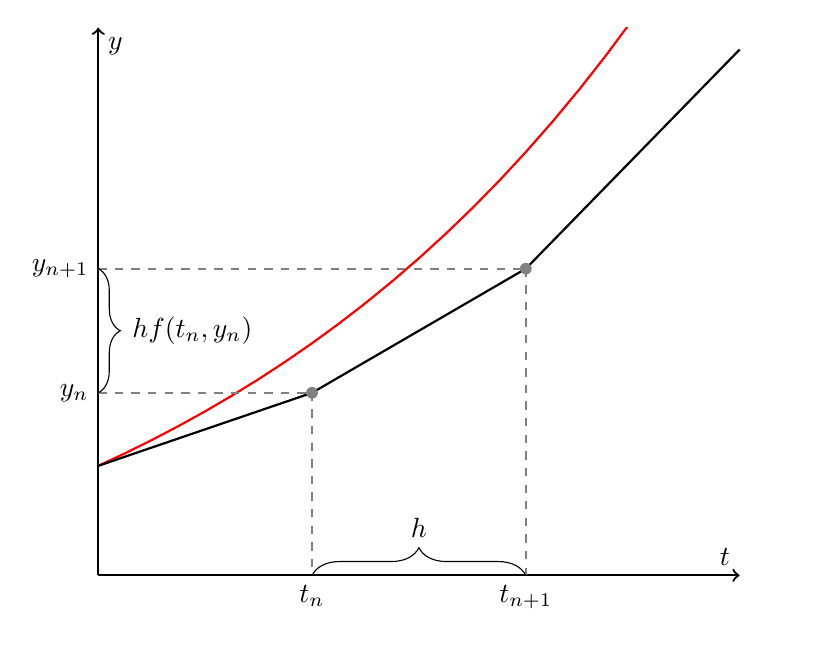
\begin{tikzpicture}
        \begin{axis}[
            %axis x line=bottom,
            %axis y line=left,
            axis x line=none,
            axis y line=none,
            height=0.75\linewidth,
            width=0.95\linewidth,
            xmin=-0.33,
            xmax=3.33,
            ymin=0.3,
            ymax=3,
        ]
        
        \addplot[thick, black, ->] coordinates {(0, 0.5) (3, 0.5)}; % x-axis
        \addplot[thick, black, ->] coordinates {(0, 0.5) (0, 3)}; % y-axis
   
        % This is not to scale, only for demonstrative purposes
        \addplot[thick, red, domain=0:3]{exp(x/2.25)};
        \addplot[thick, black] coordinates {(0, 1) (1, 1.3333)};
        \addplot[thick, black] coordinates {(1, 1.3333) (2, 1.9)};
        \addplot[thick, black] coordinates {(2, 1.9) (3, 2.9)};
       
        \addplot[thick, gray, dashed] coordinates {(1, 1.3333) (1, 0.5)}; % x=1
        \addplot[thick, gray, dashed] coordinates {(2, 1.9) (2, 0.5)}; % x=2
        
        \node[anchor=north, draw=none] at (1, 0.5) {\(t_n\)};
        \node[anchor=north, draw=none] at (2, 0.5) {\(t_{n+1}\)};
        
        \draw [decorate,decoration={brace,amplitude=10pt},xshift=0pt,yshift=0pt] (1, 0.5) -- (2, 0.5) node  [black, midway, yshift=17pt] {\(h\)};
        
        \addplot[thick, gray, dashed] coordinates {(0, 1.3333) (1, 1.3333)};
        \addplot[thick, gray, dashed] coordinates {(0, 1.9) (2, 1.9)};
        
        \node[anchor=east, draw=none] at (0, 1.3333) {\(y_n\)};
        \node[anchor=east, draw=none] at (0, 1.9) {\(y_{n+1}\)};
        
        \draw [decorate,decoration={brace,amplitude=8pt},xshift=0pt,yshift=0pt] (0, 1.9) -- (0, 1.3333)  node [black, midway, xshift=34pt] {\(hf(t_n, y_n)\)};
        
        \node[anchor=north west, draw=none] at (0, 3) {\(y\)};
        \node[anchor=south east, draw=none] at (3, 0.5) {\(t\)};
    
        \node[circle, fill, inner sep=1.5pt, gray] at (1, 1.3333){};
        \node[circle, fill, inner sep=1.5pt, gray] at (2, 1.9){};
        
        \node[circle, inner sep=0pt] at (3.33, 3){};
        
        \end{axis}
    \end{tikzpicture}
    \caption[En illustration av Eulers stegmetod.]{En illustration av Eulers stegmetod. Den röda grafen är \(y\), och den svarta är en numerisk lösning med hjälp av Eulers metod.} \label{fig:eulers-method}
\end{figure}

Eftersom \(y_0\) behöver vara känt löser Eulers metod endast så kallade begynnelsevärdes\-problem \parencite[310]{suli_introduction_2003}.

\subsubsection{Utvidgning av Eulers metod till system av differentialekvationer}\label{sec:euler_dev}
Eulers metod löser, som sagt, differentialekvationer på formen \(y'=f(t, y)\) För att lösa ett system av kopplade differentialekvationer på formen
\begin{equation}
    X'=f(t, X)
\emph{,}\end{equation} där
\begin{equation*}
    X=\pmtx{x_1\\\vdots\\x_i}
\end{equation*} och 
\begin{equation*}
    f(t, X)=\pmtx{
        f_1(t, x_1,\hdots,x_i)\\
        \vdots\\
        f_i(t, x_1,\hdots,x_i)
    }
\end{equation*}
behöver metoden emellertid utvecklas, om än lite:
\begin{equation}
    x_{i, n+1}=x_{i, n}+hf_i(t_n, x_{n, 1},\hdots,x_{n, i})
\eqph{,}\end{equation} vilket också kan skrivas 
\begin{equation}
    X_{n+1}=X_{n}+hf(t_n, X_n)
\end{equation} \parencites[340; 355-356]{atkinson_introduction_1989}.

\subsection{Heuns metod}
Heuns metod är en vidareutveckling av Eulers metod. Istället för att säga att lutningen för en steglängd är derivatan i punkt \(t_n\), tar Heuns metod även med derivatan i punkt \(t_{n+1}\), och beräknar medelvärdet av dem. Matematiskt skrivs det:
\begin{equation}
    y_{n+1}=y_n+\frac{1}{2}h(f(t_n, y_n)+f(t_{n+1}, \hat{y}_{n+1}))
\emph{,}\end{equation} där \(\hat{y}_{n+1}\) är det förutspådda värdet då \(t=t_{n}\) Detta räknas ut med Eulers metod; alltså:
\begin{equation}
     \hat{y}_{n+1}=y_{n}+hf(t_n, y_n)
\end{equation} \parencite[324]{suli_introduction_2003}. Denna kan också vidareutvecklas till system av differentialekvationer på samma sätt som i \ref{sec:euler_dev}, vilket ger:
\begin{equation}
    X_{n+1}=X_n+\frac{1}{2}h(f(t_n, X_n)+f(t_{n+1}, \hat{X}_{n+1}))
\end{equation}

\subsection{Analytisk lösning av kopplade differentialekvationer på formen \texorpdfstring{\(X'=AX+B\)}{X'=AX+B}}
Systemen på formen i (\ref{eq:coupled_ode_matrix_form}) kan lösas med hjälp av egenvärden och egenvektorer.

\subsubsection{Linjära avbildningar}
En matris kan beskriva en så kallad linjär avbildning. En avbildning är i grunden en funktion, med vektorer som definitions- och värdemängd. En 2-dimensionell linjär avbildning kan ibland illustreras genom att ``dra'' i alla punkter. En linjär avbildning är en avbildning som bevarar skalning och summor, med andra ord:
\begin{equation}
    L(k\vec{v})=kL(\vec{v})
\end{equation}
\begin{equation}
    L(\vec{v}+\vec{u})=L(\vec{v})+L(\vec{u})
\end{equation}
där \(L\) är en linjär transformation, \(k\) är en konstant, och \(\vec{v}\) samt \(\vec{u}\) är vektorer \parencite{sanderson_linear_2016}. Figur \ref{fig:linear_map} visar ett exempel på en linjär avbildning.

\begin{figure}[h!]
    \centering
    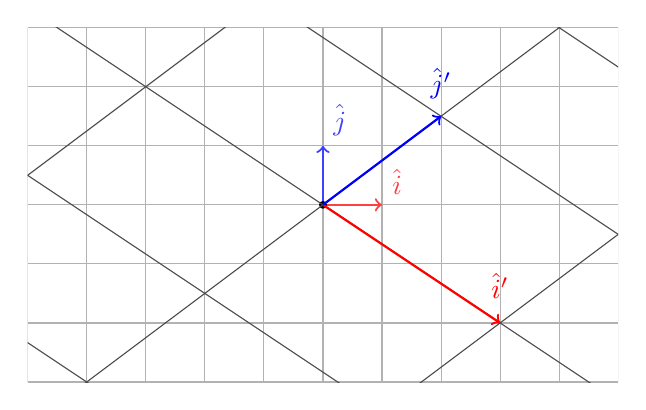
\begin{tikzpicture}[scale=0.75]
        \clip (-5,-3) rectangle (5,3);
        
        \draw[black!30] (-5,-3) grid (5,3);
        
        \draw[red!75, thick, ->] (0,0) -- (1,0) node[above right]{\(\hat{i}\)};
        \draw[blue!75, thick, ->] (0,0) -- (0,1) node[above right]{\(\hat{j}\)};
        
        \node at (0, 0) [circle,fill,inner sep=1pt]{};
        
        \begin{scope}
            \pgftransformcm{3}{-2}{2}{1.5}{\pgfpoint{0cm}{0cm}}
            
            \foreach \X in {-8,...,8}
                {\draw[black!70] (\X,-5) -- ++ (0,10);}
            
            \foreach \Y in {-4,...,4}
                {\draw[black!70] (-3,\Y) -- ++ (6,0);}
            
            \draw[red, thick, ->] (0,0) -- (1,0) node[above=0.5em]{\(\hat{i}'\)};
            \draw[blue, thick, ->] (0,0) -- (0,1) node[above=0.25em]{\(\hat{j}'\)};
        \end{scope}
        
    \end{tikzpicture}
    \caption[Exempel på en linjär avbildning.]{Exempel på en linjär avbildning. Enhetsvektorerna \(\hat{i}\) och \(\hat{j}\) är utmarkerade, samt enhetsvektorerna efter den linjära transformationen, \(\hat{i}'\) och \(\hat{j}'\). Den matrisen som beskriver denna avbildning är \(\pmtx{3&2\\-2&1.5}\).}\label{fig:linear_map}
\end{figure}

\subsubsection{Egenvärden och egenvektorer}
Om en vektor endast förändras i magnitud, alltså inte i riktning, vid en linjär avbildning kallas den vektorn för \emph{egenvektor}. Skalfaktorn för en egenvektor i en linjär avbildning kallas \emph{egenvärde}. Rent matematiskt uttrycks det som:
\begin{equation}\label{eq:eigenvalue-eigenvector-def}
    A\vec{v}=\lambda\vec{v}
\end{equation} där \(A\) är en matris, \(\vec{v}\) är en egenvektor, och \(\lambda\) är ett egenvärde. \(\vec{v}\) kan inte vara nollvektorn, eftersom det är ett trivialfall \parencites[App-14]{zill_differential_2005}[283]{strang_introduction_2009}. Om \(\lambda=1\) transformeras inte vektorn, vilket innebär att \(A=I\), där \(I\) är identitetsmatrisen. Alltså:
\begin{equation}
    A\vec{v}=\vec{v}\Rightarrow A=I=
    \pmtx{
        1 & 0 & \hdots & 0\\
        0 & 1 & \hdots & 0\\
        \vdots & \vdots & \ddots & \vdots\\
        0 & 0 & \hdots & 1
    }
\end{equation} eftersom \(I\) är enhetsavbildningen för vektorer \parencite{noauthor_identitetselement_nodate}. \(\vec{v}\) är i detta fall alla tänkbara vektorer, vilket innebär att alla vektorer är egenvektorer av \(I\) med egenvärde 1 \parencite[283]{strang_introduction_2009}.

\subsubsection{Determinanter}
\emph{Determinant} är ett värde som ges till varje kvadratisk matris, och beskriver några av dess egenskaper \parencite{noauthor_determinant_nodate}. Determinanten för en \(2\times 2\)-matris definieras:
\begin{equation}
    \det A=
    \begin{vmatrix}
    a & b\\c & d
    \end{vmatrix}
    = ad-bc
\eqph{,}\end{equation} eftersom ekvationssystemet som representeras av matrisen \(A\) saknar lösningar om \(\det A=0\). För en matris av högre dimension definieras determinanten
\begin{equation}
    \begin{split}
    \begin{vmatrix}
        a_{11} & a_{12} & a_{13} & \hdots & a_{1k}\\
        a_{21} & a_{22} & a_{23} & \hdots & a_{2k}\\
        a_{31} & a_{32} & a_{33} & \hdots & a_{3k}\\
        \vdots & \vdots & \vdots & \ddots & \vdots\\
        a_{k1} & a_{k2} & a_{k3} & \hdots & a_{kk}
    \end{vmatrix}=
    a_{11}\begin{vmatrix}
        a_{22} & a_{23} & \hdots & a_{2k}\\
        a_{32} & a_{33} & \hdots & a_{3k}\\
        \vdots & \vdots & \ddots & \vdots\\
        a_{k2} & a_{k3} & \hdots & a_{kk}
    \end{vmatrix}\\-a_{12}\begin{vmatrix}
        a_{21} & a_{22} & \hdots & a_{2k}\\
        a_{31} & a_{32} & \hdots & a_{3k}\\
        \vdots & \vdots & \ddots & \vdots\\
        a_{k1} & a_{k2} & \hdots & a_{kk}
    \end{vmatrix}+\hdots\pm a_{1k}\begin{vmatrix}
        a_{21} & a_{22} & \hdots & a_{2(k-1)}\\
        a_{31} & a_{32} & \hdots & a_{3(k-1)}\\
        \vdots & \vdots & \ddots & \vdots\\
        a_{k1} & a_{k2} & \hdots & a_{k(k-1)}
    \end{vmatrix}
    \end{split}
\end{equation} \parencite{weisstein_determinant_nodate}. Determinanter är väldigt användbara inom exempelvis linjär algebra, matematisk analys, och lösningar till linjära ekvationssystem \parencites{weisstein_determinant_nodate}{noauthor_determinant_nodate}.

Determinanten kan därutöver geometriskt tolkas som skalfaktorn för en area vid en linjär avbildning, som demonstreras i figur \ref{fig:det_linear_transformation} \parencite{sanderson_determinant_2016}.

\begin{figure}[h!]
    \centering
    \begin{subfigure}[b]{0.49\textwidth}
    \centering
    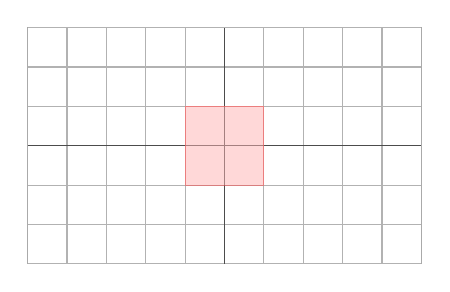
\begin{tikzpicture}[scale=0.5]
        \clip (-5,-3) rectangle (5,3);
        \draw[black] (-5,-3) rectangle (5,3);
        
        \draw[black!30] (-5,-3) grid (5,3);

        \draw[black!70] (-5, 0) -- (5, 0);
        \draw[black!70] (0, -3) -- (0, 3);
        
        \draw[color=red!70, fill=red!30, opacity=0.5] (-1, -1) rectangle (1,1);
        
    \end{tikzpicture}
    \caption{Före linjär avbildning. \(\mathrm{Area}=a\)}
    \end{subfigure}
    \hfill
    \begin{subfigure}[b]{0.49\textwidth}
    \centering
    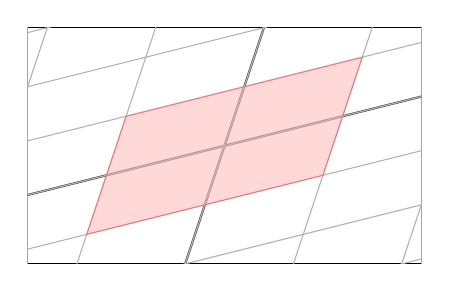
\begin{tikzpicture}[scale=0.5]
        \clip (-5,-3) rectangle (5,3);
        \draw[black] (-5,-3) rectangle (5,3);
        
        \begin{scope}
            \pgftransformcm{0.5}{1.5}{3}{0.75}{\pgfpoint{0cm}{0cm}}

            \draw[black!70, thick] (0, -5) -- (0, 5);
            \draw[black!70, thick] (-3, 0) -- (3, 0);
            
            \foreach \X in {-8,...,8}
                {\draw[black!30] (\X,-5) -- ++ (0,10);}
            
            \foreach \Y in {-4,...,4}
                {\draw[black!30] (-3,\Y) -- ++ (6,0);}
            
            \draw[color=red!70, fill=red!30, opacity=0.5] (-1, -1) rectangle (1,1);
        \end{scope}
        
    \end{tikzpicture}
    \caption{Efter linjär avbildning. \(\mathrm{Area}=a\det A\)}
    \end{subfigure}
    
    \caption{Determinanten kan geometriskt tolkas som den faktor som en area skalas med vid en linjär avbildning.}\label{fig:det_linear_transformation}
\end{figure}

\subsubsection{Att finna egenvärden och egenvektorer}\label{sec:eigenvalues_vectors}
(\ref{eq:eigenvalue-eigenvector-def}) kan omskrivas till \(A\vec{v}-\lambda\vec{v}=0\). Vidare kan \(\vec{v}\) multipliceras med identitesmatrisen och faktoriseras, vilket ger
\begin{equation}
    (A-\lambda I)\vec{v}=\vec{0}
\end{equation} \parencite[247]{margalit_interactive_2019}. Om båda sidor multipliceras med \((A-\lambda I)^{-1}\) ges
\begin{equation}
    (A-\lambda I)^{-1}(A-\lambda I)\vec{v}=\vec{0}(A-\lambda I)^{-1}
\eqph{.}\end{equation} Denna kan förenklas till
\begin{equation}
    \vec{v}=\vec{0}
\eqph{.}\end{equation} \(\vec{v}\) kan inte vara lika med nollvektorn, och därför kan inte \(A-\lambda I\) vara inverterbar. Detta innebär som följd att dess determinant måste vara lika med noll, eftersom alla ekvationssystem med lösningar är inverterbara. Det vill säga
\begin{equation}
    \det(A-\lambda I)=0
\end{equation} \parencite[286-287]{strang_introduction_2009}. Denna kallas ofta för en matris \emph{karakteristiska ekvation}, och dess lösningar är matrisens egenvärden \parencite[338]{zill_differential_2005}.

Egenvektorer erhålles genom att lösa \((A-\lambda I)\vec{v}=0\), med de uträknade egenvärdena \parencite{kuttler_71_2022}. Till exempel har matrisen
\begin{equation*}
    \pmtx{
        2 & 3\\
        1 & 4
    }
\end{equation*}
egenvärdena 1 och 5. För att finna egenvektorerna löses \((A-\lambda I)\vec{v}=0\) en gång per egenvärde. För \(\lambda_1\) är ekvationen
\begin{equation}
    \left(\bmtx{
        2 & 3\\
        1 & 4
    }
    -1I\right)\vec{v}=\pmtx{
        1 & 3\\
        1 & 3
    }
    \pmtx{x_1\\x_2}=\vec{0}
\eqph{.}\end{equation} Detta är ett homogent linjärt ekvationssystem, och kan därför lösas med Gausselimination. I detta fall subtraherar vi rad 1 från rad 2. Alltså
\begin{equation}
    \begin{array}({@{}cc|c@{}})
        1 & 3 & 0 \\
        1 & 3 & 0
    \end{array}
    \rightarrow
    \begin{array}({@{}cc|c@{}})
        1 & 3 & 0 \\
        0 & 0 & 0
    \end{array}
\end{equation}
Det ger att \(x_1+3x_2=0\), vilket i sin tur ger att \(x_1=-3x_2\). Detta innebär vidare att
\begin{equation}
    \vec{v}=\pmtx{
        -3x_2\\
        x_2
    }
\end{equation} Detta är egenvektorn för egenvärdet 1. Denna vektor är invariant över en linjär transformation, oavsätt magnitud. \(x_2\) är därför en godtycklig skalär. Den kan till  exempel sättas till 1:
\begin{equation}
    \vec{v}=\pmtx{-3\\1}
\end{equation}
Denna process upprepas med de övriga egenvärdena \parencite{kuttler_71_2022}.

\subsubsection{Superpositionsprincipen}
Superpositionsprincipen, ibland kallad linjäritetsprincipen, säger att om \(y_1\), \(y_2\hdots\) \(y_n\) är oberoende lösningar av en homogen linjär differentialekvationer är
\begin{equation}
    y=c_1y_1+c_2y_2+\hdots+c_ny_n
\end{equation} ännu en lösning, där \(c\) är konstanter \parencite[130]{zill_differential_2005}. Denna gäller även för ett system av differentialekvationer, där
\begin{equation}
    X=c_1X_1+c_2X_2+\hdots+c_nX_n
\end{equation} är en lösning, om \(X_1\), \(X_2\hdots\) \(X_n\) är oberoende lösningar \parencite[249]{blanchard_differential_2010}.
%Superpositionsprincipen innebär att om två signaler (funktioner) adderas och matas in genom ett filter (funktion), är resultatet densamma som om två signaler hade matats igenom filtret separat och sedan adderats \parencite{smith_superposition_nodate}. Detta kan appliceras på differentialekvationer. Om oberoende lösningar av en homogen linjär differentialekvation har erhållits kan en mer generell lösning skrivas
%\begin{equation}
%    y=c_1y_1+c_2y_2+\hdots+c_ny_n
%\end{equation} där \(c_n\) är konstanter, \(y_n\) är oberoende lösningar, och \(n=1,2,3\hdots\) \parencite[130]{zill_differential_2005}. I ett inhomogent linjärt system gäller att
%\begin{equation}
%    y=c_1y_1+c_2y_2+\hdots+c_ny_n+y_p
%\end{equation} där \(y_p\) är en partikulärlösning \parencite[336]{zill_differential_2005}.

\subsubsection{Lösningsformel}
Vi antar att \(X=Ke^{\lambda t}\) är en lösning till differentialekvationerna \(X'=AX\), där \(K\) är en kolonnvektor med samma dimension som \(X\) och \(\lambda\) är en konstant. Vidare innebär detta att \(X'=(Ke^{\lambda t})'=K\lambda e^{\lambda t}\). Detta leder till att \(K\lambda e^{\lambda t}=AKe^{\lambda t}\). \(e^{\lambda t}\) kan sedan divideras bort, vilket ger att \(AK=\lambda K\)  \parencite[338]{zill_differential_2005}. Denna är ekvivalent med (\ref{eq:eigenvalue-eigenvector-def}), och vi kan därför använda matematiken i avsnitt \ref{sec:eigenvalues_vectors} för att erhålla lösningar.

Om egenvärdena är reella är den generella lösningen således
\begin{equation}                      
    X(t)=c_1K_1e^{\lambda_1t}+c_2K_2e^{\lambda_2t}+\hdots+c_nK_ne^{\lambda_nt}
\end{equation}
där \(c\) är konstanter, \(K_1, K_2, \hdots K_n\) egenvektorerna, och \(\lambda_1, \lambda_2, \hdots \lambda_n\) egenvärdena.
Om egenvärderna istället är komplexa kan formeln ovan skrivas
\begin{equation}\label{eq:complex_eigenvalues_solution}
    X(t)=c_1K_1e^{(\alpha+i\beta)t}\hdots=c_1K_1e^{\alpha t} e^{i\beta t}\hdots
\eqph{.}\end{equation}
Med hjälp av Eulers formel kan denna sedan omskrivas till
\begin{equation}
    X(t)=c_1K_1e^{\alpha t}(\cos\beta t + i\sin\beta t)\hdots
\eqph{.}\end{equation} Den karakteristiska ekvationen har alltid konjugerade par som lösningar om koefficienterna är reella. Detta innebär att \(\overbar{K}e^{\overbar{\lambda}t}\) är en lösning om \(Ke^{\lambda t}\) är en lösning \parencite[342]{zill_differential_2005}. Således är
\begin{equation}
    X(t)=c_1\overbar{K_1}e^{\overbar{\lambda_1}t}\hdots=c_1\overbar{K_1}e^{(\alpha-i\beta)t}\hdots
\end{equation} också en lösning. Denna kan, likt ovan, skrivas
\begin{equation}
    X(t)=c_1\overbar{K_1}e^{\alpha t}(\cos\beta t - i\sin\beta t)\hdots
\end{equation} \parencite[347-348]{zill_differential_2005}. Superpositionsprincipen innebär att
\begin{equation}
    X=c_1X_1+c_2X_2\cdots
\eqph{,}\end{equation} där \(c_i\) är konstanter, \(X_i\) är lösningar, \(i=1,2,3\cdots\), och \(X\) är en ny lösningsvektor \parencite[333]{zill_differential_2005}. Genom superpositionsprincipen kan (\ref{eq:complex_eigenvalues_solution}) skrivas
\begin{equation}
    X(t)=c_1K_1e^{\lambda_1 t}+c_2\overbar{K_1}e^{\overbar{\lambda_1}t}
\eqph{.}\end{equation} Konstanterna kan sedan multipliceras in i egenvektorerna, vilket ger
\begin{equation}
    X(t)=K_1e^{\lambda_1 t}+\overbar{K_1}e^{\overbar{\lambda_1}t}
\eqph{.}\end{equation} För att underlätta kan egenvektorerna även multipliceras med \(\frac{1}{2}\), vilket i sin tur ger
\begin{equation}
    \begin{split}
        X(t)&=\frac{1}{2}(K_1e^{\lambda_1 t}+\overbar{K_1}e^{\overbar{\lambda_1}t})\\
        &=\left(\frac{1}{2}(K_1+\overbar{K_1})\cos\beta t-\frac{i}{2}(K_1+\overbar{K_1})\sin\beta t\right)e^{\alpha t}
    \end{split}
\eqph{.}\end{equation}
Dessutom är 
\begin{equation}
    \begin{split}
        X(t)&=\frac{i}{2}(-K_1e^{\lambda_1 t}-\overbar{K_1}e^{\overbar{\lambda_1}t})\\
        &=\left(\frac{i}{2}(-K_1+\overbar{K_1})\cos\beta t+\frac{1}{2}(K_1+\overbar{K_1})\sin\beta t\right)e^{\alpha t}
    \end{split}
\end{equation} en lösning, genom samma metod. Dessa kan skrivas
\begin{equation}
    \begin{split}\label{eq:sol_of_ode_complex_eigenvalues}
        X(t)&=(B_1\cos\beta t-B_2\sin\beta t)e^{\alpha t}\\
        X(t)&=(B_2\cos\beta t+B_1\sin\beta t)e^{\alpha t}
    \end{split}
\end{equation} där
\begin{equation}
    \begin{split}
        B_1&=\frac{1}{2}(K_1+\overbar{K_1})=\Re(K_1)\\
        B_2&=\frac{i}{2}(-K_1+\overbar{K_1})=\Im(K_1)
    \end{split}
\end{equation} \parencite[348]{zill_differential_2005}. En mer generell lösning kan följaktligen skrivas
\begin{equation}\label{eq:general_sol_of_ode_complex_eigenvalues}
    X=X_1+X_2+\hdots X_k
\eqph{,}\end{equation} där \(k\) är antalet egenvärden och -vektorer, enligt superpositionsprincipen. För ett system med två beroende variabler blir den generella lösningen alltså
\begin{equation}
    X=X_1+X_2
\end{equation}

\subsubsection{Begynnelsevillkor}
Ekvation \ref{eq:general_sol_of_ode_complex_eigenvalues} kan, enligt superpositionsprincipen, utvecklas till
\begin{equation}
    X=c_1 X_1 + c_2 X_2\hdots c_k X_k
\eqph{,}\end{equation} där \(c\) är konstanter \parencite[332-333]{zill_differential_2005}. Genom att sätta \(X(0)\) ekvation till en vektor med initialvärderna bildas ett ekvationssystem, som kan lösas. Om begynnelsevillkoren till exempel var 2 respektive 1 i en tvådimensionell kolonnvektor hade ekvationssystemet sett ut
\begin{equation}
    aX_1(0)+bX_2(0)=
    \pmtx{2\\1}
\eqph{.}\end{equation} På så sätt kan \(a\) och \(b\) bestämmas, så värdena då \(t=0\) är initialvärderna \parencite[348-349]{zill_differential_2005}.

\subsubsection{Inhomogena differentialekvationer}
System på formen
\begin{equation}
    X'=AX
\end{equation} kallas \emph{homogena}. System på formen
\begin{equation}\label{eq:inhomogeneous_ode}
    X'=AX+B
\end{equation} kallas således \emph{inhomogena}. Lösningen till en inhomogen differentialekvation ges av
\begin{equation}\label{eq:sol_of_inhomogeneous_ode}
    X=X_c+X_p
\eqph{,}\end{equation} där \(X_c\) är den motsvarande homogena differentialekvationens lösning, som kan fås genom metoden som beskrivs ovan, och \(X_p\) är en partikulärlösning \parencites[336]{zill_differential_2005}[188]{alfredsson_matematik_2013}. En partikulärlösning är en vektor, \(X\), som uppfyller (\ref{eq:inhomogeneous_ode}) \parencite[335]{zill_differential_2005}.

För att finna en partikulärlösning behöver dess form först bestämmas. Detta arbete kommer endast beröra \(B\) som konstanta vektorer, och därför kommer formen av \(X_p\) antas vara
\begin{equation}
    X_p=\begin{pmatrix}
        \alpha\\\beta
    \end{pmatrix}
\eqph{.}\end{equation}
Denna kan sedan substitueras in i (\ref{eq:inhomogeneous_ode}), vilket ger
\begin{equation}
    \vec{0}=A\begin{pmatrix}
        \alpha\\\beta
    \end{pmatrix}+B
\eqph{.}\end{equation} Således skapas ett ekvationssystem, som kan lösas, vars lösningar är \(\alpha\) och \(\beta\).

\subsubsection{Periodicitet}
Eftersom komplexa egenvärden genererar lösningar med trigonometriska funktioner genererar de stundtals sinusodiala kurvor, och är därmed stundom periodiska. Om \(e^{\alpha t}=1\), det vill säga \(\Re(\lambda)=0\), kommer lösningens termer endast innehålla trigonometriska funktioner samt konstanter, och är därmed periodiska \parencite[398]{zill_differential_2005}. Determinanten av \(A-I\lambda\) är
\begin{equation}
    \begin{vmatrix}
        a-\lambda & b\\
        c & d-\lambda
    \end{vmatrix}
    = \lambda^2-(a+d)\lambda+(ad-bc)
\eqph{.}\end{equation} Rötterna av denna ekvation är således
\begin{equation}
    \lambda=\frac{1}{2}(a+d)\pm \sqrt{\frac{1}{4}(a+d)^2-(ad-bc)}
\eqph{.}\end{equation} För att \(\Re(\lambda)=0\) måste \(\frac{1}{2}(a+d)=0\), vilket kan omskrivas till \(a=-d\). Dessutom måste \(-(ad-bc)<0\) för att \(\Im(\lambda)\neq0\). Denna olikhet kan skrivas \(bc-ad<0\). Om \(ad\) adderas till båda sidor ges \(bc<ad\). Eftersom \(a=-d\), kan det substitueras in: \(bc<a(-a)\Leftrightarrow bc<-a^2\). Båda sidor kan sedan multipliceras med \(-1\), och olikhetstecknets vänds därmed: \(-bc>a^2\). Det måste alltså finnas två villkor på matrisen för periodicitet, vilka är:
\begin{equation}\label{eq:conditions_periodicty}
    \begin{cases}
        a=-d\\
        a^2<-bc
    \end{cases}
\end{equation}

%\subsubsection{Matrisexponentialfunktioner}
%Det går även att lösa linjära kopplade differentialekvationer med hjälp av \(e\). Differentialekvationen
%\begin{equation*}
%    y'=ry
%\end{equation*} där \(r\) är en konstant har lösningen
%\begin{equation}
%    y=Cre^t
%\end{equation} där \(C\) är en konstant, som motsvaras av begynnelsevillkoret \parencite[185]{alfredsson_matematik_2013}. Detta resonemang går att generalisera till matriser. Ponera istället den kopplade differentialekvationen
%\begin{equation*}
%    \pmtx{x'\\y'}=\pmtx{a&b\\c&d}\pmtx{x\\y}
%\eqph{.}\end{equation*} Denna kommer ha lösningen
%\begin{equation}
%    \pmtx{x\\y}=Ce^{\pmtx{a&b\\c&d}}
%\end{equation} där \(C\) är en tvådimensionell kolonnvektor med begynnelsevillkoren \parencite[171]{bellman_introduction_1997}. För att höja upp \(e\) i en matris måste först Taylorutvecklingen definieras:
%\begin{equation}
%    e^x=1+x+\frac{x^2}{2!}+\frac{x^3}{3!}\cdots
%\end{equation} \parencite{rowland_matrix_nodate}. I grunden är \(e^x\) endast definierade för \(x\in\mathbb{R}\), och därför används beteckningen \(\exp(x)\) för \(e^x\) där \(x\notin\mathbb{R}\) \parencite[170]{bellman_introduction_1997}. Genom att beräkna värdet för Taylorutvecklingen med en viss matris kan en lösning därmed erhållas. I detta arbete kommer emellertid endast egenvärde-egenvektor-metoden användas.

\subsubsection{Exempellösning av ett system}
För att sammanfatta löses systemet
\begin{equation}
    X'=\pmtx{4&16\\-2&-4}X,\qquad X(0)=\begin{pmatrix}1\\1\end{pmatrix}
\eqph{.}\end{equation} Först räknas egenvärderna ut:
\begin{equation}
    \det(A-\lambda I)=\begin{vmatrix}
        4-\lambda&16\\-2&-4-\lambda
    \end{vmatrix}=\lambda^2+16=0\Rightarrow\lambda=\pm 4i
\end{equation}
Eftersom egenvärderna är konjugerande par behöver endast ett tas hänsyn till. För att finna egenvektorerna löses \((A-\lambda I)\vec{v}=0\):
\begin{equation}
    (A-\lambda I)\vec{v}=\pmtx{4-4i&16\\-2&-4-4i}\pmtx{x\\y}=\pmtx{(4-4i)x+16y\\-2x-(4+4i)y}=\pmtx{0\\0}
\eqph{.}\end{equation} Genom att subtrahera rad två från rad ett erhålles
\begin{equation}
    (2-4i)x+(8-4i)y=0
\eqph{.}\end{equation} \(x\) kan sedan lösas ut till
\begin{equation}
    x=(2-2i)y
\end{equation} och \(y\) sätts till \(1\), vilket ger
\begin{equation}
    \vec{v}=\pmtx{2-2i\\1}=\pmtx{2\\1}+\pmtx{-2\\0}i
\eqph{.}\end{equation} Därefter används ekvation \ref{eq:sol_of_ode_complex_eigenvalues}, vilket ger
\begin{equation}
    X_1(t)=\left(\pmtx{2\\1}\cos(4t)-\pmtx{-2\\0}\sin(4t)\right)e^{0t}
\end{equation}
\begin{equation}
    X_2(t)=\left(\pmtx{-2\\0}\cos(4t)+\pmtx{2\\1}\sin(4t)\right)e^{0t}
\eqph{.}\end{equation} Enligt superpositionsprincipen kan en mer generell lösning skrivas
\begin{equation}
    X(t)=a\left(\pmtx{2\\1}\cos(4t)-\pmtx{-2\\0}\sin(4t)\right)+b\left(\pmtx{-2\\0}\cos(4t)+\pmtx{2\\1}\sin(4t)\right)
\eqph{.}\end{equation}
\(X(0)\) sätts därefter till begynnelevillkoren:
\begin{equation}
\begin{split}
    X(0)&=a\left(\pmtx{2\\1}\cos(0)-\pmtx{-2\\0}\sin(0)\right)+b\left(\pmtx{-2\\0}\cos(0)+\pmtx{2\\1}\sin(0)\right)\\
    &=a\pmtx{2\\1}+b\pmtx{-2\\0}=\pmtx{1\\1}
\end{split}
\eqph{.}\end{equation} Då bildas ekvationssytemet
\begin{equation}
    \begin{cases}
        2a-2b=1\\
        a=1
    \end{cases}
\end{equation} som löses till
\begin{equation}
    \begin{cases}
        a=1\\
        b=0.5
    \end{cases}
\eqph{,}\end{equation} vilket innebär att lösningen till differentialekvationen är
\begin{equation}
    X(t)=\left(\pmtx{2\\1}\cos(4t)-\pmtx{-2\\0}\sin(4t)\right)+\frac{1}{2}\left(\pmtx{-2\\0}\cos(4t)+\pmtx{2\\1}\sin(4t)\right)
\end{equation} Denna kan omskrivas till
\begin{equation}
    \begin{cases}
        x=2\cos(4t)+2\sin(4t)-\cos(4t)+\sin(4t)\\
        y=\cos(4t)+\frac{1}{2}\sin(4t)
    \end{cases}
\eqph{,}\end{equation} som i sin tur kan förenklas till
\begin{equation}
    \begin{cases}
        x=\cos(4t)+3\sin(4t)\\
        y=\cos(4t)+\frac{1}{2}\sin(4t)
    \end{cases}
\end{equation}

\subsection{Avvikelser i numeriska lösningsmetoder}\label{sec:error_analysis}
Det finns flera källor till avvikelser i numeriska lösningsmetoder. Nedan följer ett urval av dem.

\subsubsection{Avrundnings- och flyttalsfel}
Datorer har begränsat minne, och kan därför bara lagra tal till en viss precision. Dessutom kan inte alla tal representeras exakt i binär form. Exempelvis kommer en dator påstå att \(0.1+0.2\neq0.3\), eftersom \(0.1\) och \(0.2\) inte kan representeras exakt i binär form: \(0.1_\text{tio}=0.0001100110011_\text{två}\cdots\) och \(0.2_\text{tio}=0.001100110011_\text{två}\cdots\). Då uppstår ett avrundningsfel, vilket leder till det tidigare nämnda fenomenet \parencite[20]{atkinson_introduction_1989}.

\subsubsection{Tunkeringsfel}
När ett problem löses numeriskt kommer avvikelser oundvikligen uppstå (Se figur \ref{fig:truncation-error}). Dessa samlas under begreppet \emph{trunkeringsfel} (ibland kallat \emph{diskretiseringsfel}) \parencite[20; 342]{atkinson_introduction_1989}. Till exempel kan \(\frac{1}{1-x}\) approximeras med Taylorutvecklingen
\begin{equation*}
    \frac{1}{1-x}=1+x+x^2+x^3\cdots
\end{equation*} då \(|x|<1\) \parencite{math_is_fun_taylor_nodate}. Om endast 3 termer används för approximationen, det vill säga
\begin{equation*}
    \frac{1}{1-x}\approx1+x+x^2
\eqph{,}\end{equation*} är trunkeringsfelet
\begin{equation*}
    \frac{1}{1-x}-(1+x+x^2)=x^3+x^4+x^5\cdots
\end{equation*}

\begin{figure}[h!]
    \centering
    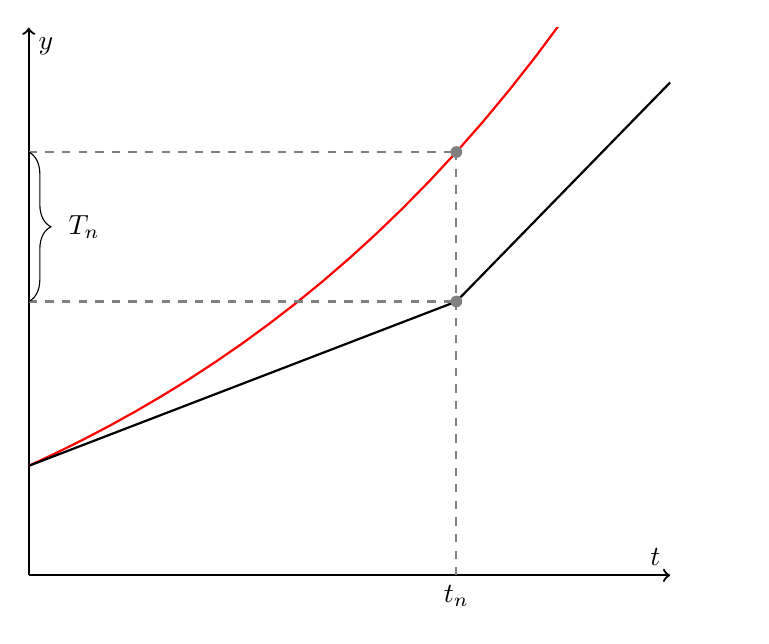
\begin{tikzpicture}
        \begin{axis}[
            %axis x line=bottom,
            %axis y line=left,
            axis x line=none,
            axis y line=none,
            height=0.75\linewidth,
            width=0.95\linewidth,
            xmin=-0.33,
            xmax=3.33,
            ymin=0.3,
            ymax=3,
        ]
        
        \addplot[thick, black, ->] coordinates {(0, 0.5) (3, 0.5)}; % x-axis
        \addplot[thick, black, ->] coordinates {(0, 0.5) (0, 3)}; % y-axis
   
        % This is not to scale, only for demonstrative purposes
        \addplot[thick, red, domain=0:3]{exp(x/2.25)};
        \addplot[thick, black] coordinates {(0, 1) (2, 1.75)};
        \addplot[thick, black] coordinates {(2, 1.75) (3, 2.75)};
       
        \addplot[thick, gray, dashed] coordinates {(2, 2.43242545) (2, 0.5)};
        
        \node[anchor=north, draw=none] at (2, 0.5) {\(t_n\)};
                
        \addplot[thick, gray, dashed] coordinates {(0, 1.75) (2, 1.75)};
        \addplot[thick, gray, dashed] coordinates {(0, 2.43242545) (2, 2.43242545)};
                
        \draw [decorate,decoration={brace,amplitude=8pt},xshift=0pt,yshift=0pt] (0, 2.43242545) -- (0, 1.75)  node [black, midway, xshift=20pt] {\(T_n\)};
        
        \node[anchor=north west, draw=none] at (0, 3) {\(y\)};
        \node[anchor=south east, draw=none] at (3, 0.5) {\(t\)};
    
        \node[circle, fill, inner sep=1.5pt, gray] at (2, 1.75){};
        \node[circle, fill, inner sep=1.5pt, gray] at (2, 2.43242545){};
        
        \node[circle, inner sep=0pt] at (3.33, 3){};
        
        \end{axis}
    \end{tikzpicture}
    \caption[En visualisering av trunkeringsfelet.]{En visualisering av trunkeringsfelet. \(T_n\) är trunkeringsfelet vid tidpunkten \(t_n\).} \label{fig:truncation-error}
\end{figure}


\subsubsection{Ordo-notation}
Det kan vara hjälpsamt att introducera så kallad ordo-notation. Om \(e(h)\) betecknar trunkeringsfelet som en funktion av steglängden, och det finns en konstant \(C\) sådant att
\begin{equation}
    |e(h)|\leq Ch^n
\end{equation} för tillräckligt små \(h\) är \(e(h)\) av order \(n\), och betecknas \(\ordo(h^n)\). Om steglängden halveras ges
\begin{equation}\label{eq:ordo_half_h}
    C(\frac{h}{2})^n=Ch^2\frac{1}{2^n}\geq\frac{1}{2^n}e(h)
\eqph{.}\end{equation} Med andra ord minskar felet maximalt med \(1/2^n\) då \(h\) är tillräckligt liten \parencite[369-370]{zill_differential_2005}.

\subsubsection{Medelvärdessatsen och Taylors teorem}
Medelvärdessatsen kommer visa sig användbar i vissa härledningar. Differensen mellan två funktionsvärden kan, enligt den, skrivas
\begin{equation}
    \frac{f(b)-f(a)}{b-a}=f'(\xi)
\end{equation} där \(f\) är en kontinuerlig funktion, \(a\) och \(b\) är punkter och \(\xi\) är en punkt inom intervallet \((a, b)\) \parencite[235]{atkinson_numerical_2009}. Beviset utelämnas från denna text; se \textcite[141]{adams_calculus_2010}. Den generaliserade medelvärdessatsen lyder
\begin{equation}\label{eq:general_mean_value_theorem}
    \frac{f(b)-f(a)}{g(b)-g(a)}=\frac{f'(\xi)}{g'(\xi)}
\end{equation} för de kontinuerliga funktionerna \(f\) och \(g\) där \(g'(x)\neq 0\) för alla \(x\) inom intervallet \((a, b)\) \parencite[141]{adams_calculus_2010}. Ett bevis för den generaliserade medelvärdessatsen finnes i bilaga \ref{proof_generalised_mvt}.

Inom många härledningar kommer även Taylorutvecklingar användas. Enligt den kan en kontinuerlig funktion \(f(x)\) uttryckas
\begin{equation}
    f(x)=p_n(x)+R_{n}(x)
\end{equation} där
\begin{equation}
    p_n(x)=f(x_0)+\frac{x-x_0}{1!}f'(x_0)+\frac{(x-x_0)^2}{2!}f''(x_0)+\cdots+\frac{(x-x_0)^n}{n!}f^{(n)}(x_0)
\end{equation} där \(x_0\) och \(x\) är en punkter på ett visst intervall, samt
\begin{equation}
    R_{n}(x)=\frac{(x-x_0)^{n+1}}{(n+1)!}f^{(n+1)}(\xi)
\end{equation} där \(\xi\) är en punkt mellan \(x_0\) och \(x\), förutsatt att funktionen är deriverbar \(n+1\) gånger \parencite[236]{atkinson_numerical_2009}. Ett bevis för resttermen i Taylors teorem finnes i bilaga \ref{proof_taylors_theorem}.

\subsubsection{Trunkeringsfelet i Eulers metod}
Trunkeringsfelet i Eulers metod på analytisk form kan härledas med hjälp av en Taylorutveckling. \(X(t)\) kan skrivas som
\begin{equation}\label{eq:taylor_series_x_def}
    X(t)=\left(\sum_{n=0}^k X^{(n)}(a)\frac{(t-a)^n}{n!}\right)+R_{n}(t)
\eqph{,}\end{equation} alltså
\begin{equation}
    X(t)=X(a)+X'(a)\frac{t-a}{1!}+\cdots+X^{(n)}(a)\frac{(t-a)^n}{n!}+R_{n}(t)
\eqph{,}\end{equation} där \(a\) är en punkt nära \(t\), \(n\) är en konstant och \(R_{n}\) är resten, enligt Taylors teorem. \(R_n\) kan i sin tur skrivas som
\begin{equation}
    R_{n}(t)=X^{(n+1)}(\xi)\frac{(t-a)^{n+1}}{(n+1)!}
\eqph{,}\end{equation} där \(\xi\) är en punkt mellan \(a\) och \(x\). Om \(n=1\), \(a=t\) och \(t=t_{n+1}=t_n+h\) kan (\ref{eq:taylor_series_x_def}) skrivas som
\begin{equation}
    \begin{split}
        X(t_{n+1})&=X(t)+X'(t)h+R_{n}\\
        &=X(t)+X'(t)h+X''(c)\frac{h^2}{2}
    \end{split}
\eqph{.}\end{equation} Eftersom \(X(t)=X_n\) och \(X'=f(t_n, X_n)\) kan ekvationen ovan skrivas som
\begin{equation}
    X(t_{n+1})=X_n+hf(t_n, X_n)+X''(c)\frac{h^2}{2}
\eqph{.}\end{equation} Notera att \(X_n+hf(t_n, X_n)\) är Euler's metod (jämför med ekvation \ref{eq:eulers_method_def}). Detta gör att ekvationen kan skrivas
\begin{equation}
    X(t_{n+1})=X_{n+1}+X''(c)\frac{h^2}{2}
\eqph{.}\end{equation} Trunkeringsfelet kan således uttryckas
\begin{equation}
    T_n=X''(c)\frac{h^2}{2}=Ch^2
\eqph{,}\end{equation} där \(c\) är en punkt mellan \(X_n\) och \(X_{n+1}\) och \(C\) är en konstant. \parencite[369]{zill_differential_2005}. \(c\) är svårt att ta reda på, och därför är trunkeringsfelet i stort sätt aldrig känt, eftersom det skulle ge en exakt lösning.

Trunkeringsfelet är således av graden 2, alltså \(\ordo(h^2)\).

\subsubsection{Trunkeringsfelet i Heuns metod}
Trunkeringsfelet i Heuns metod kan härledas på liknande sätt som för Eulers metod till \(\ordo(h^3)\) \parencite[372]{zill_differential_2005}. För bevis, se \textcite[113-114]{atkinson_numerical_2009}. Detta innebär som följd att en halvering i steglängden i Heuns metod leder till en maximal minskning av trunkeringsfelet till en åttondel av dess tidigare värde, enligt (\ref{eq:ordo_half_h}).

\subsubsection{Globala trunkeringsfelet}
Varje punkt \(y_{n+1}\) innehåller trunkeringsfel från punkten \(y_n\), men \(y_n\) innehåller i sin tur ett trunkeringsfel från \(y_{n-1}\) och så vidare. Trunkeringfelet mellan två punkter kallas \emph{lokala trunkeringsfelet}, och är det som diskuterats tidigare. Det totala trunkeringsfelet kallas \emph{globala trunkeringsfelet}, ofta betecknat \(\tau_n\) eller \(e_n\), och är en summation av trunkeringsgfelet för alla tidigare steg \parencite[370]{zill_differential_2005}.

För att härleda det globala trunkeringsfelet i Eulers metod definieras först \(e_{n+1}=y(t_{n+1})-n_{n+1}\) och \(e_n=y({t_n})-y_n\). Enligt Eulers metod kan \(y(t_{n+1})\)
skrivas
\begin{equation}\label{eq:derivation_tau_euler_exact}
    y(t_{n+1})=y(t_n)+hf(t_n, y(t_n))+T_n
\end{equation} där \(T_n\) är det lokala trunkeringsfelet. \(y_{n+1}\) kan även skrivas
\begin{equation}\label{eq:derivation_tau_euler_approx}
    y_{n+1}=y_n+hf(t_n, y_n)
\eqph{.}\end{equation} Om (\ref{eq:derivation_tau_euler_approx}) subtrahetas från (\ref{eq:derivation_tau_euler_exact}) ges
\begin{equation}
    y(t_{n+1})-y_{n+1}=(y(x_n)+hf(t_n, y(t_n))+T_n)-(y_n+hf(t_n, y_n))
\end{equation}
vilket ger
\begin{equation}\label{eq:e-n+1-eulers}
    e_{n+1}=e_n+h(f(t_n, y(t_n))-f(t_n, y_n))+T_n
\eqph{.}\end{equation} \(T_n\) definieras
\begin{equation}
    T_n\leq kh^2
\end{equation} där \(k\) är en konstant. Låt \(M\) beteckna det maximala värdet som \(k\) kan anta, alltså \(\mathrm{max}(k)\). Då kan (\ref{eq:e-n+1-eulers}) skrivas
\begin{equation}\label{eq:en-inequality}
    |e_{n+1}|\leq |e_n|+h|f(t_n, y(t_n))-f(t_n, y_n)|+Mh^2
\eqph{.}\end{equation} Med hjälp av medelvärdessatsen fås
\begin{equation}
    f(t_n, y(t_n))-f(t_n, y_n)=f_y(t_n, c)(y(t_n)-y_n)=f_y(t_n, c)e_n
\eqph{,}\end{equation} där \(c\) antar ett värde mellan \(y(t_n)\) och  \(y_n\). Detta innebär som följd att
\begin{equation}
    |f(t_n, y(t_n))-f(t_n, y_n)|\leq R|e_n|
\eqph{,}\end{equation} där \(R\) är en konstant. Genom att kombinera ekvationen ovan samt (\ref{eq:en-inequality}) fås
\begin{equation}\label{eq:e-n+1-factorised}
        |e_{n+1}|\leq |e_n|+h|Re_n|+Mh^2
\eqph{,}\end{equation} vilket kan faktoriseras till
\begin{equation}
    |e_{n+1}|\leq (1+Rh)|e_n|+Mh^2
\eqph{.}\end{equation} Antag att \(e_0=0\). \(e_1\) kan således anta ett maximalt värde av \(Mh^2\). Om (\ref{eq:e-n+1-factorised}) appliceras iterativt ges
\begin{equation}\label{eq:error-iterative}
    \begin{split}
        |e_1|\leq& Mh^2\\
        |e_2|\leq& (1+Rh)|e_1|+Mh^2 \leq (1+(1+Rh))Mh^2\\
        |e_3|\leq& (1+Rh)|e_2|+Mh^2 \leq (1+(1+Rh)+(1+Rh)^2)Mh^2\\
        \vdots&\\
        |e_n|\leq& (1+Rh)|e_{n-1}|+Mh^2 \leq (1+(1+Rh)+\cdots +(1+Rh)^{n-1})Mh^2
    \end{split}
\end{equation} Notera att \(1+(1+Rh)+(1+Rh)^2\cdots\) är en geometrisk serie, och kan därför skrivas
\begin{equation}
    \frac{(1+Rh)^n-1}{Rh}
\eqph{.}\end{equation} Om denna kombineras med (\ref{eq:error-iterative}) ges
\begin{equation}\label{eq:e-n-leq-w-1+rh}
    |e_n|\leq \frac{(1+Rh)^n-1}{R}Mh
\eqph{.}\end{equation} \(1+Rh\leq e^{Rh}\) för alla värden på \(Rh\)\footnote{\textit{Bevis:} Betrakta funktionen \(f(x)=e^x-(1+x)\). Då är \(f'(x)=e^x-1\). För att \(f'(x)=0\) måste \(x=0\). \(f''(x)=e^x\), och \(f''(0)=1\), vilket innebär en minimipunkt då \(x=0\). Värdemängden för \(f(x)\) är således \(f(x)\geq 0\). \(\square\)}, vilket leder till
\begin{equation}
    (1+Rh)^n\leq e^{nRh}
\eqph{.}\end{equation} Denna kan substitueras in i (\ref{eq:e-n-leq-w-1+rh}), vilket ger
\begin{equation}
    |e_n|\leq \frac{(e^{nRh})-1}{R}Mh
\eqph{.}\end{equation} \(nh=t_n\), vilket innebär att föregående ekvation kan skrivas
\begin{equation}
    |e_n|\leq \frac{(e^{t_nR})-1}{R}Mh=\frac{(Me^{t_nR})-M}{R}h
\eqph{.}\end{equation} Således är
\begin{equation}
    |e_n|\leq Ch
\eqph{,}\end{equation} där \(C\) är en konstant, vilket innebär att ordo-notationen för det globala trunkeringsfelet i Eulers metod är \(\ordo(h)\) \parencites{trench_31_2020}{feldman_d22_nodate}. Detta kan sedan generaliseras till slutsatsen att det globala trunkeringsfelet har ordo-notationen \(\ordo(h^{n-1})\) om det lokala trunkeringsfelet har ordo-notationen \(\ordo(h^n)\) \parencite[370]{zill_differential_2005}. Det globala trunkeringsfelet i Heuns metod är alltså \(\ordo(h^2)\).

\subsection{Tidigare forskning}
\textcite[344-345]{atkinson_introduction_1989} fann att trunkeringsfelet ungefär halveras vid en halvering av steglängden i Eulers metod, i två differentialekvationer:
\begin{equation*}
    y'=e^x\quad\mathrm{samt}\quad y'=2x
\end{equation*} med steglängderna \(h=0.2\), \(h=0.1\) och \(h=0.05\) i fem punkter: \(x=0.4\), \(x=0.8\), \(x=1.2\), \(x=1.6\) och \(x=2.0\). \textcite[320-321]{suli_introduction_2003} drog liknande slutsatser. De undersökte systemet
\begin{equation*}
    y'=y+g(x)
\end{equation*} där
\begin{equation*}
    g(x)=\frac{x^4+6x^3+12x^2-14x+9}{(1+x^2)}
\end{equation*} med samma steglängder som \citeauthor{atkinson_introduction_1989}, och fann att trunkeringsfelet minskar med cirka en faktor av två vid halveringen av steglängden i Eulers metod. \textcite[371]{zill_differential_2005} undersökte systemet
\begin{equation*}
    y'=2xy
\end{equation*} med steglängder \(h=0.1\) och \(h=0.05\). De drog slutsatsen att en halvering av av trunkeringsfelet sker med en halverad steglängd i Eulers metod. De undersökte även samma system och steglängder med Heuns metod, där de fann att trunkeringsfelet minskar med en faktor av ungefär fyra vid en halvering av steglängden.

\textcite{pratiwi_eulers_2021} undersökte skillnaden mellan Eulers och Heuns metod i en smittspridningsmodell av COVID-19. De fann att skillnaden var försumbar, trots att Heuns metod i teorin är signifikant mer noggrann.
